
\setvruler[][][][3][0]
\chapter{Introduction}
\pagenumbering{arabic}
\setcounter{page}{1}

This document specifies a collection of compiler
directives, runtime library routines that can be used to specify
distributed-memory parallel programming in \C and \Fort
program. These define the specification of \XMP Application
Program Interface (\XMP API). This specification provides a
model of parallel programming for distributed memory multiprocessor
systems. The directives extend the \C and \Fort base languages as to
describe distributed memory parallel program.

\section{Scope}

\XMP API
is used to explicitly specify the action to be taken by the compiler
and runtime system to execute the parallel program in distributed
memory system. \XMP-compliant implementations are not required
to check for invalid local data access, data conflicts, racing
conditions, or deadlock. The \XMP is defined by following items:

\begin{itemize}
\item A Set of directives
\item Minimum language extension on base languages (\C and \Fort)
\item Runtime libraries
\item Environment Variables
\end{itemize}

\section{Features of \XMP}

Features of \XMP are summarized as follows:

\begin{description}
\item {\bf Language extensions} for familiar languages \C and \Fort,
  which can reduce code-rewriting and educational costs.
\item \XMP supports typical parallelization based on the {\bf data parallel
  paradigm} and work sharing under {\it global view}, and enables
  parallelizing the original sequential code using minimal
  modification with simple {\bf directives}, like \OMP. 
\item \XMP also includes CAF-like PGAS (Partitioned
Global Address Space) feature as {\it local view} programming. 
\item {\bf Explicit communication and synchronization}. All actions
  are taken by directives for being ``easy-to-understand'' for
  performance-aware programming.
\item For flexibility and extensibility, the execution model
allows {\bf combining with explicit \MPI coding} for more complicated
and tuned parallel codes and libraries. 
\item For multi-core and SMP clusters,
{\bf \OMP directives can be combined} into \XMP for thread
programming inside each node as a hybrid programming
model.
\end{description}

\XMP is being designed based on the experiences of \HPF, Fujitsu XPF
(VPP FORTRAN) and OpenMPD.  

\chapter{Overview of \XMP model and language}

\section{Hardware model and execution model}

The target of \XMP is a distributed memory system
(Figure \ref{fig1}). Each compute node, which may have
several cores sharing main 
memory, has its own local memory, and each node is connected via
network. Each node can access and modify its local memory directly,
and can access the memory on the other nodes via communication. It
is however assumed that accessing remote memory is much slower than
the access of local memory.

The basic execution model of
\XMP is a SPMD (Single Program Multiple Data) model on
distributed memory. In each node, a program starts from the same main
routine. An \XMP program begins as a single thread of execution
in each node. 

When the thread encounters \XMP directives,
the synchronization and communication occurs between nodes. That is,
no synchronization and communications happen without directives. In
this case, the program does duplicated execution of the same program
on local memory in each node.

\OMP API can be used in order to
make use of multicores in a node. In this specification, we define
actions only when one thread executes \XMP directives at a
time.

\begin{myfigure}
\includegraphics[width=12cm]{figs/Fig1.eps}
  \caption{Hardware Model}\label{fig1}
\end{myfigure}

As default, data
declared in the program is allocated in each node, and is referenced
locally by threads executed in the node. 

\XMP supports two
models of viewing data: global-view programming model and local-view
programming model. In local-view programming model, accesses to data
in remote nodes are done explicitly by language extension for get/put
operations on remote nodes with node number of the target nodes, while
reference to local data is executed implicitly. 

In contrast to
the local-view programming mode, a global-view programming model is
one in which programmers express their algorithm and data structure as
a whole, mapping them to the node set. The programmers describe the
data distribution and the work mapping to express how to distribute
data and share the work among nodes. The variables in global-view
programming model look like a shared memory spanning over
nodes.

\section{Global-view programming model}

The global-view
programming model is useful when, starting from sequential version of
the program; the programmer parallelizes it in data-parallel model by
adding directives incrementally with minimum modifications.In the
global-view programming model, the programmer describes the data
distribution of data shared among the nodes by data distribution
directives. {\tt loop} construct maps works in iterations to the node where
computed data is located. Global-view communication directives are
used to synchronize between nodes, keep the consistency of shadow
area, and move a part of distributed data globally. It should be noted
that the programmer must keep all data reference required computations
done locally by any appropriate directives. 

In many cases, the
\XMP program using the global-view is based on a sequential
program and able to produce the same result independent from the
number of compute nodes (Figure \ref{fig2}). The
global view provides a 
programming model in which computation and data are distributed onto
compute nodes.

There are three groups of directives for the
global-view programming model. As these directives can be ignored as a
comment by the compilers of base languages (\C and \Fort), an
\XMP program derived from a sequential program can preserve the
integrity of original program when it is run sequentially. 

\subsubsection*{Data Mapping}
Specify Data distribution and mapping to nodes (partially
inherited from HPF)

\subsubsection*{Work Mapping (Parallelization)}
Assign works to nodes. {\tt loop} construct map each iteration to
nodes where the referenced elements are located, and Task construct
execute each task parallel in different node set.

\subsubsection*{Communication and Synchronization}
Describe how to communicate and synchronize with the other compute
nodes. In \XMP, the inter-node communication must be described
explicitly. The compiler guarantees that communication takes place
only if communication is explicitly specified.

\begin{myfigure}
\includegraphics[width=12cm]{figs/Fig2.eps}
  \caption{Parallelization by global-view programming model}
\label{fig2}
\end{myfigure}

\section{Local-view programming model}

Local view is suitable for the
programs explicitly describing the algorithm of each node and explicit
remote data reference (Figure \ref{fig3}). As MPI is
considered to have the local 
view, the local view programming model of \XMP has high
interoperability with MPI.

For the local view programming model,
the language extension and some directives are provided. The coarray
notation taken from \CAF (CAF) is such an extension. For
example, to access an array element of {\tt A(i)} located on compute
node {\tt N},
the expression of {\tt A(i)[N]} is used. If the access is a value reference,
then the communication to get the value takes place. If the access is
updating the value, then the communication to put a new value takes
place.

\begin{myfigure}
\includegraphics[width=12cm]{figs/Fig3.eps}
  \caption{Local-view programming model}
\label{fig3}
\end{myfigure}

\section{Interactions between global-view and local-view}

The node in
\XMP is used to distribute data or distribute computational
load. In local view, the node is used in conjunction with the coarray
directive to reference data. In the application program, programmers
should choose an appropriate data model according to the structure of
the program. Figure \ref{fig4} illustrates global-view and
local-view of data.

Data may have a global view and local view and can be
accessed from a global view or local view. \XMP provides some
directives to put local name (alias) to the global data declared in
global-view programming mode so that the data can be referenced also
in local-view programming model. It may be useful to optimize the
program by explicit remote data reference in local-view programming
model.

\begin{myfigure}
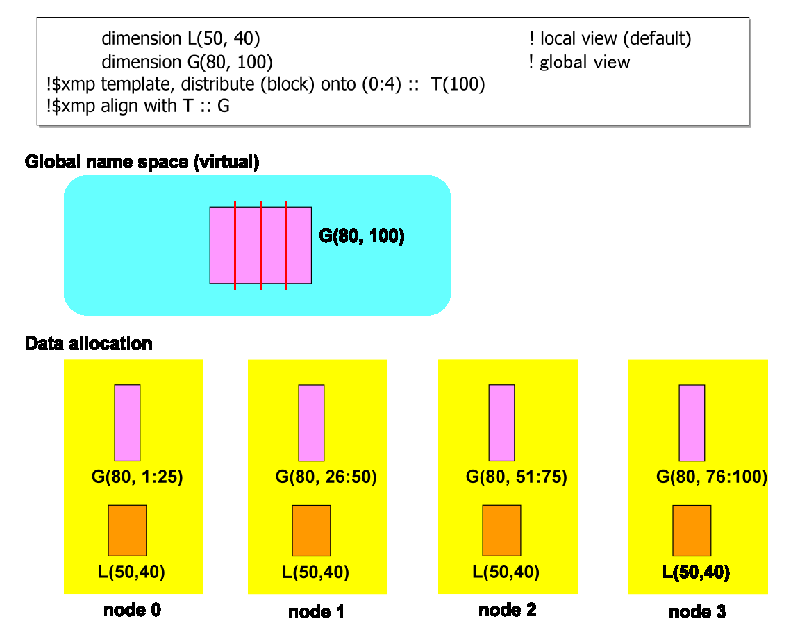
\includegraphics[width=12cm]{figs/Fig4.eps}
  \caption{Global view and local view}
\label{fig4}
\end{myfigure}

\section{Execution model and Task}


In \XMP, a program begins as a single thread
of execution in each node. The set of nodes when starting a program is
called entire nodes.

A task is a specific instance of executable
code and its data environments executed in a set of nodes. A task when
starting a program in entire nodes is called an initial task. The
initial task can generate a subtask which executes on a subset of the
nodes by {\tt task} construct. A set of nodes executing the same task is
called executing nodes. If no {\tt task} construct is encountered, a
program is executed as one task, and its executing nodes are entire
nodes.

As far as no directives are encountered, a program executes
locally. When the same codes are executed, almost same computation is
performed in each node, called duplicated execution. When the threads
encounter {\tt loop} construct or {\tt array} construct, the specified
loop is executed in parallel so that each iteration is assigned to the
node where specified data element is located. 

A new task is generated by
{\tt task} construct. A code in the {\tt task} construct is executed
as a subtask executed in a specified node set. When a subroutine is
called in the context of the task, the subroutine is executed on its
executing nodes. 

For synchronization and communications between nodes, a set of
directives are provided. In local view programming model, a coarray
features are adopted for remote data reference. It should be noted
that all synchronization and communication are specified by directives
explicitly, and without such directives, no communications are
executed implicitly by the compiler.
